\documentclass[a4paper, 12pt]{scrartcl}



\usepackage[utf8]{inputenc}

\usepackage[english]{babel}
\usepackage{amssymb}
\usepackage[T1]{fontenc}
\usepackage{mathtools}
\usepackage{amsmath}
\usepackage{ntheorem}
\usepackage{bbm}
\usepackage{dsfont}
\usepackage{color}
\usepackage{slashed}
\usepackage{hyperref}
\usepackage{graphicx} 
\usepackage{bm}
\usepackage{mathabx}
\usepackage{multirow}
\usepackage{float}
\begin{document}
\begin{titlepage}
	\centering
	{\scshape\LARGE University of Tübingen \par}
	\vspace{2cm}
	{\huge\bfseries Thermionic Emission \par}
	\vspace{2cm}
	{\Large \scshape Blockpraktikum 2021} \par
	\vspace{2cm}
	{\Large  First English Version} \par
	\vspace{2cm}
	{\Large\itshape \underline{David Schütz} \space \space  \underline{Christian Gommeringer}\par}
	\vfill 
	{\large overlooked by Jia Tang}
	\vfill

	{\large \today\par}
\end{titlepage}
\newpage 
\tableofcontents 

\newpage
\section{Introduction} 
In this experiment we analyse the behavior of a glowing diode emitting electrons which is the so called thermionic emission. At first we start with the theoretical fundamentals by describing the problem with the laws of physics. Then we hand over by describing the experiment and it´s implementation. Further we evaluate our measurements and present our result. 
\newline 
\newline 
\section{Theoretical Fundamentals} 
A part of the electrons in the reverse-bias domain have enough energy to overcome the work function potential and aswell the small reverse bias voltage 
\begin{align}
U_{\textrm{AK}} = \varphi_\textrm{A} - \varphi_\textrm{K} = -U_\textrm{G}(\varphi_\textrm{A}, \varphi_\textrm{K}) 
\end{align}
where $\varphi_\textrm{K}$ is the cathode potential and $\varphi_{A}$ is the anode potential. ($U_\textrm{G} > 0$) The starting current is given by 
\begin{align}
I_\textrm{A}(U_\textrm{G},T) = I_\textrm{S}(T) \cdot  \exp \left( - \frac{eU_\textrm{G}}{k_\textrm{B}T} \right) 
\end{align}
where $I_\textrm{S}(T)=I_\textrm{A}(0,T)$ is the saturation current, $e$ the elementary charge, $k_\textrm{B}$ the Boltzmann-constant, $T$ cathode temperature. Due to Sommerfeld and Nordheim we have an expression of the saturation current in dependence of the cathode temperatur $T$ and the cathode work function $W_\textrm{K}$. Without an external field it yields to
\begin{align}
\textrm{I}_\textrm{S} (T) = A_0 FT^2 \exp \left( - \frac{W_\textrm{K}}{k_\textrm{B} T} \right)
\end{align}
with a constant $A_0$ and the surface area of the cathode $F$. The tube in the experiment has the radii ratio of anode radii and cathode radii  $\frac{R}{r} \approx 1,5$, which is important for the homogene surface with temperature independent work function. It guarantees us the validity of equation (3). For cathodes which are not fullfilling this condition, is it possible to calculate with the Richardson-equation 
\begin{align}
\textrm{I}_\textrm{S} (T) = A_\textrm{R} FT^2 \exp \left( - \frac{W_\textrm{K}}{k_\textrm{B} T} \right)
\end{align}
\newline 
\newline 
When we are taking the natural logarithm of $I_\textrm{A}$ and also plotting this versus $U_\textrm{G}$, it is possible to calculate the cathode temperature out of the slope of the resultating line. But the applied reverse voltage needs to be corrected cause of two effects. First, the space charge between cathode and anode forms a potential barrier in the near of the cathode. Second, the diffrence between the work functions of cathode and anode is resulting in a contact voltage between cathode and anode. 
\newline 
\newline 
For small current densities is the spacecharge minor and can be neglected. The effective reverse bias voltage is in due consideration of the contact potential given by 
\begin{align}
U_{\textrm{AK}}^{\textrm{eff}} = -U_\textrm{G} + \frac{1}{e}(W_\textrm{K}-W_\textrm{A})
\end{align}
with the work functions of cathode $W_\textrm{K}$ and anode $W_{\textrm{A}}$. With this we obtain then 
\begin{align}
I_\textrm{A} (U_\textrm{G},T) = A_0 F T^2 \exp \left( - \frac{W_\textrm{A} + e U_\textrm{G}}{k_\textrm{B} T } \right)
\end{align}
When the influence of the cathode temperature $T$ on the work function $W_\textrm{A}$ is minor, it is then possible to calculate $T$ out of (6). For the anode work function $W_\textrm{A}$ we find
\begin{align}
W_\textrm{A} = k_\textrm{B} T \cdot \ln \left( \frac{A_0 F T^2}{I_\textrm{A}(0,T)} \right)
\end{align}
The calculation of the cathode work function is in our case redundant. 
\section{Experiment Execution}
The experimental setup is clarified by following picture. 
\begin{figure}[H]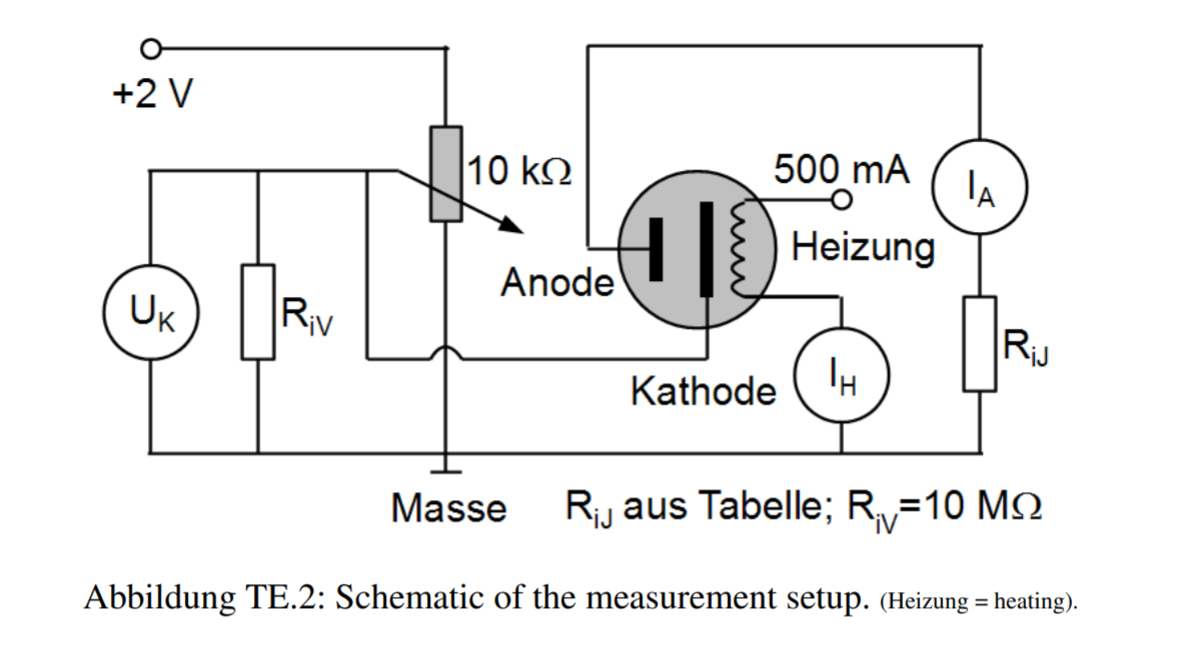
\includegraphics[scale=0.7]{TEpic1}\caption{circuit design for our experiment from the instructions}\end{figure}
We build this setup and let it check from the assistant. Then we measured for diffrent heating currents ($I_\textrm{H} = 450,500,550 \textrm{mA}$) the measurment series $I_\textrm{A} = I_\textrm{A}(U_\textrm{G})$. Further we increased the reverse bias Voltage from 0V in 20 equidistant steps until we measured a starting current $I_\textrm{A} \leq 2$nA. Each time we measured the starting current $I_\textrm{A}$ we also note the measurement range of the digital multimeter. This is important for the evaluation of our measurements. The dependence of the internal resistance of our measuring device from the measurement range is depicted in the following table.

\begin{figure}[H]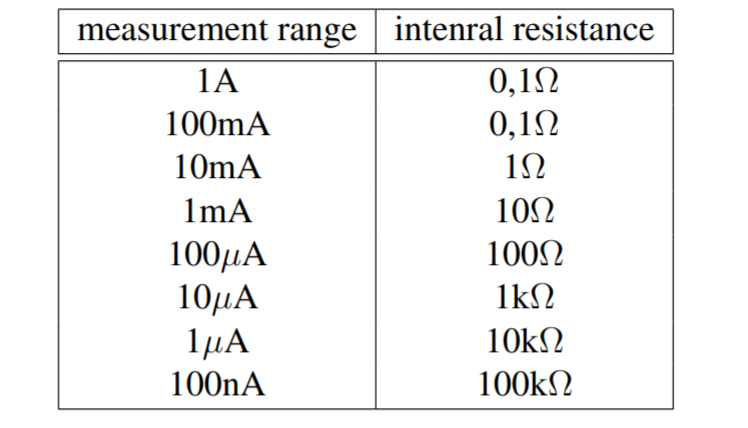
\includegraphics[scale=1]{TEpic2}\caption{internal resistance for each measurement range; source: instruction paper of this experiment}\end{figure}

\newpage
\section{Analysis of the measurement results}

We determined the dependence of the starting current $I_A$ from the reverse bias voltage for three different heating currents.
\begin{table}[H]\begin{tabular}{ccccccccccc}
$U_\text{tot}$ in $V$&0&0.098&0.2&0.3&0.398&0.5&
0.599&
0.65&
0.7&
0.751\\
$I_A$ in $A$&142&
147&
120&
116&
84&
62.5&
34.9&
24.1&
15.5&
8.4\\m. r.&1mA&
1mA&
1mA&
1mA&
1mA&
100µA&
100µA&
100µA&
100µA&
10µA\\&&&&&&&&&&\end{tabular}\newline
\hspace*{-2cm}\begin{tabular}{ccccccccccccc}
$U_\text{tot}$ in $V$&0.801&
0.85&
0.901&
0.951&
1.001&
1.05&
1.098&
1.149&
1.199&
1.25&
1.349&
1.4\\
$I_A$ in $A$&5.15&
2.94&
1.66&
0.845&
0.498&
0.276&
0.159&
0.0939&
0.049&
0.027&
0.0053&
0.0011\\
m. r.&10µA&
10µA&
10µA&
1µA&
1µA&
1µA&
1µA&
1µA&
1µA&
100nA&
100nA&
100nA\end{tabular}\caption{measurement with $I_H=450\,mA$ heating current (m.r. stands for the used measurement range)}\end{table}

\begin{table}[H]\begin{tabular}{ccccccccccc}$U_\text{tot}$ in $V$&0&
0.065&
0.131&
0.194&
0.259&
0.324&
0.39&
0.454&
0.521&
0.585\\
$I_A$ in $A$&361&
286&
221&
162.9&
109.8&
68.5&
40.3&
22.9&
12.36&
6.61\\
m. r.&1mA&
1mA&
1mA&
100µA&
100µA&
100µA&
100µA&
100µA&
10µA&
10µA\\
&&&&&&&&&&\end{tabular}\newline
\begin{tabular}{ccccccccccc}
$U_\text{tot}$ in $V$&0.65&
0.714&
0.77&
0.786&
0.845&
0.91&
0.974&
1.04&
1.102&
1.165\\
$I_A$ in $A$&3.35&
1.69&
0.9&
0.759&
0.389&
0.184&
0.087&
0.0405&
0.0194&
0.0094\\
m. r.&10µA&
1µA&
1µA&
1µA&
1µA&
100nA&
100nA&
100nA&
100nA&
100nA\\
&&&&&&&&&&\end{tabular}
\newline
\begin{tabular}{ccc}$U_\text{tot}$ in $V$&1.23&
1.294\\
$I_A$ in $A$&0.0042&
0.0018\\
m. r.&100nA&
100nA\end{tabular}\caption{measurement data with a heating current of $I_H=500\,mA$}\end{table}

\begin{table}[H]\begin{tabular}{ccccccccccc}
$U_\text{tot}$ in $V$&0&
0.101&
0.201&
0.301&
0.402&
0.5&
0.599&
0.701&
0.8&
0.9\\
$I_A$ in $\mu{A}$&1250&
1080&
896&
748&
609&
481&
362&
253&
161&
82.2\\
m. r.&10mA&
10mA&
1mA&
1mA&
1mA&
1mA&
1mA&
1mA&
1mA&
100µA\\&&&&&&&&&&\end{tabular}\newline
\hspace*{-1cm}\begin{tabular}{cccccccccccc}
$U_\text{tot}$ in $V$&1.001&
1.101&
1.2&
1.299&
1.399&
1.499&
1.6&
1.65&
1.701&
1.75&
1.801\\
$I_A$ in $\mu{A}$&36.1&
13.7&
4.71&
1.72&
0.575&
0.0207&
0.0743&
0.0404&
0.0212&
0.0085&
0.0012\\
m. r.&100µA&
100µA&
10µA&
10µA&
1µA&
1µA&
100nA&
100nA&
100nA&
100nA&
100nA\end{tabular}
\caption{measurement data from the heating with $I_H=550\,mA$}\end{table}



In Order to use the right Voltage $U_G$ we have to take into consideration, that the voltage, we measured,($U_\text{tot}$) was the voltage, which was applied to both, cathode and anode as well as our measuring device for the starting current. It holds 
\begin{equation*}U_\text{tot}=U_G+U_\text{MC}=I\left(R_G+R_\text{MC}\right),\end{equation*}
where $I=I_A$ and the index MC denotes the current measuring device. Thus we get our real $U_G$ by applying the correction
\begin{equation*}U_G=U_\text{tot}-I_A\cdot{R_\text{MC}}\end{equation*}
After doing this we can now evaluate our data further. From Equation (6) we can derive the following expression by taking the logarithm.
\begin{equation*}\text{ln}(I_A)=-\frac{e}{k_BT}\,U_G+\text{ln}\left(A_0FT^2\right)-\frac{W_A}{k_BT}\end{equation*}
From this we can determine the temperature of the heating diode by fitting a linear regression to our data, what was done in the following.
\begin{figure}[H]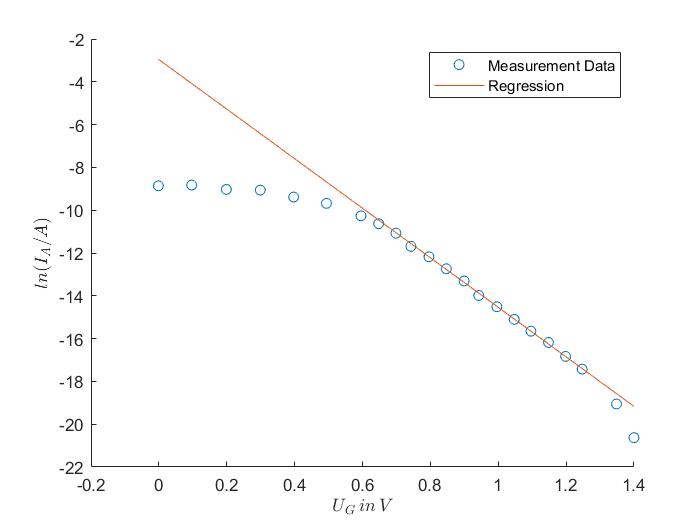
\includegraphics[scale=0.65]{450 Bild}\caption{experiment data with regression in an appropriate part with heating of $I_H=450\,mA$}\end{figure}
We approximated a function of the form $\text{ln}(I_A)=m\cdot{U_G}+b$, where $m$ was determined to 
\begin{gather*}m=-11.5769\pm0.1198\,(stat.)\pm0.0179\,(sys.)\\
b=-2.9619\pm0.1236\,(\text{stat.})\pm0.0153\,(\text{sys.}).\end{gather*} 
The calculated temperature of this result is 
\begin{equation*}T=1.0024\cdot10^3\pm10.3739\,(stat.)\pm1.5519\,(sys.)\,K.\end{equation*}
For the next heating current we proceeded the same way.

\begin{figure}[H]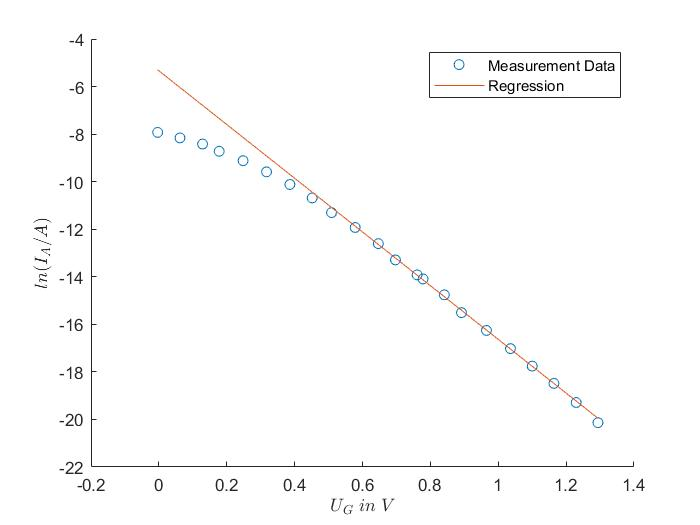
\includegraphics[scale=0.65]{500 Bild}\caption{experiment data with regression in an appropriate part with heating of $I_H=500\,mA$}\end{figure}
Out of the regression of the form $\text{ln}(I_A)=m\cdot{U_G}+b$ with
\begin{gather*}m=-11.2951\pm0.1087\,(\text{stat.})\pm0.0214\,(\text{sys.})\\
b=-5.3383\pm0.0982\,(\text{stat.})\pm0.0127\,(\text{sys.})\end{gather*}
we calculated the temperature of the heating diode as
\begin{equation*}T=1027.38\pm9.88\,(\text{stat.})\pm1.95\,(\text{sys.})\;K.\end{equation*}

\begin{figure}[H]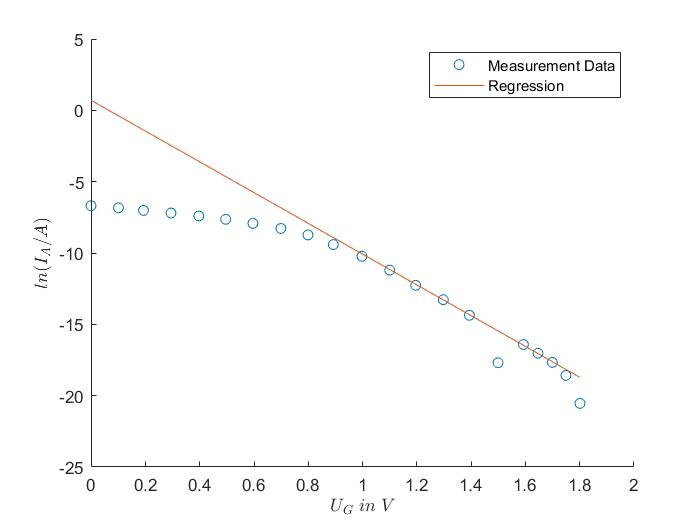
\includegraphics[scale=0.65]{550 Bild}\caption{experiment data with regression in an appropriate part with heating of $I_H=550\,mA$}\end{figure}
With the same calculation as before we calculated from the regression $\text{ln}(I_A)=m\cdot{U_G}+b$ with
\begin{gather*}m=-10.7785\pm0.1564\,(\text{stat.})\pm0.0101\,(\text{sys.})\\b=0.6933\pm0.2399\,(\text{stat.})\pm0.0158\,(\text{sys.})\end{gather*}
the temperature of the heating diode as
\begin{equation*}T=1076.64\pm15.63\,(\text{stat.})\pm1.00\,(\text{sys.})\;K.\end{equation*}


\newpage
In the next step we want to determine the anode work function $W_A$ from the equation 
\begin{equation*}W_A=k_BT\,\text{ln}\left(\frac{A_0FT^2}{I_A(0,T)}\right).\end{equation*}
The constants are given as $A_0=0.1\,\frac{A}{cm^2K^2};\:F=1.26\,cm^2$.
For $I_A(0,T)$ we take the y-axis intercept b, because our model, from which we get this formula, demands a linear course and doesn't account the effects, that lead to the deviation of the linear course. Thus we use $I_A(0,T)=exp(b)$.\newline
From this we get the result for the anode escape work from our first execution of the experiment with a heating current of $I_H=450\,mA$
$$W_{A,1}=1.2707\pm0.0175\,(\text{stat.})\pm0.0034\,(\text{sys.})\;eV$$
From a heating current of $I_H=500\,mA$ we get
$$W_{A,2}=1.5172\pm0.017\,(\text{stat.})\pm0.004\,(\text{sys.})\;eV$$
and from a heating current of $I_H=550\,mA$ we get
$$W_{A,3}=1.0390\pm0.0620\,(\text{stat.})\pm0.0052\,(\text{sys.})\;eV.$$
We calculated the statistical deviation always according to Gauß' law of error propagation
\begin{equation*}\Delta{f}\left(x_1,\dots,x_n\right)_\text{stat}=\sqrt{\sum_{i=1}^n\,\left(\frac{\partial{f}}{\partial{x_i}}\left(x_1,\dots,x_n\right)\cdot\Delta{x_i}\right)^2}\end{equation*}
and the executed the systematic error propagation over
\begin{equation*}\Delta{f}\left(x_1,\dots,x_n\right)_\text{sys}=\sum_{i=1}^n\,\left\vert\frac{\partial{f}}{\partial{x_i}}\left(x_1,\dots,x_n\right)\cdot\Delta{x_i}\right\vert\end{equation*}
As it can be seen in our results, the anode escape work is not constant, but depends slightly on the temperature of the heating diode.\newline\newline
\newpage
At this point I want to calculate, which degree of emission efficiency a diode of two different materials can get at a distinct emission current. The emitting diode shall deliver an emission current density of $j_S=0.5\,\frac{A}{cm^2}$. We consider two different cathode materials. 
At the one hand an tungsten cathode with the values $A_R=60\,\frac{A}{cm^2\,K^2},\;W_K=4.53\,eV$, and at other hand an oxide cathode with parameters $A_R=0.046\,\frac{A}{cm^2\,K^2},\;W_K=1.2\,eV$. In order to get the needed temperature for a current density of $j_S=0.5\,\frac{A}{cm^2}$, I solved the equation
\begin{equation*}j_S=A_R\,T^2\,e^{-\frac{W_K}{k_BT}}\end{equation*}
numerically and obtained the values
\begin{gather*}T_t=2565.8\,K\\T_o=1183.5\,K\end{gather*}
The power, which is applied by the diode can be calculated, according to the Stefan-Boltzmann law with emissivities $\epsilon_t=0.29$ and $\epsilon_o=0.19$
\begin{equation*}\frac{P_H}{F}=\sigma\,\epsilon\,T^4\end{equation*}
where $F$ is the surface of the cathode. We obtain
\begin{gather*}\frac{P_{H,t}}{F}=71.276\,\frac{W}{cm^2}\\\frac{P_{H,o}}{F}=2.114\,\frac{W}{cm^2}\end{gather*}
This results in a emission efficiency of
\begin{align*}\eta_t&=\frac{I_{S,t}}{P_{H,t}}=\frac{j_{S,t}}{P_{H,t}/F}=0.007\,\frac{1}{V}\\
\eta_o&=0.237\,\frac{1}{V}\end{align*}
It becomes clear that the oxide cathode is much more efficient than the tungsten one.
\newpage
\subsection{Schottky-Effect}
At the end of our Analysis I want to make a quick digression and explain the Schottky-Effect. A electron outside a metal experiences an attractive force from this metal due to electric influence. This can be described by a mirroring charge. The force on this electron in distance $r$ is expressed by
\begin{equation*}F(r)=-\frac{e^2}{4\pi\epsilon_0\,(2r)^2}\end{equation*}
In order to obtain the work, that has to be performed to remove an electron from the metal, we have to integrate this force after following rule
\begin{equation*}W=-\int_{0}^\infty\,F\,\text{d}r\end{equation*}
The electrons already got an energy in the metal due to Pauli's principle, the Fermi energy. Therefore they don't have to muster the whole escape work i.e. from thermal energy. To account this fact I start the integration from particular point $R_F$, which depends on the Fermi energy, and is therefore material dependent.
\begin{equation*}W=-\int_{R_F}^\infty\,F\,\text{d}r\end{equation*}
When in this situation an additional constant electric field is applied, which supports the escaping movement of the electron by its polarization, then the force turns at some point $r_0$ from an attractive to a repulsive force. The potential has a maximum at this point and the work, which brings the electron to this point, has to be performed in order to remove the electron from the metal. To determine the position of $r_0$ we solve the equation
\begin{equation*}0=-\frac{e^2}{16\pi\epsilon_0\,r_0^2}-e\,E\end{equation*}
We find
\begin{equation*}r_0=\sqrt{-\frac{e}{16\pi\epsilon_0\,E}}\end{equation*}
We also see that the sign of the electric field has to be negative in order to be able to notice this effect. Further we can say, that the larger the electric field is the closer comes the maximum of the potential to the surface of the metal. We notice a difference in the escape work of the electron with this additional electric field in form of
\begin{align*}\Delta{W}&=-\int_0^\infty\,F\left(r,E=0\right)\,\text{d}r\;+\int_0^{r_0}\,F(r,E)\,\text{d}r\\
&=-\int_{r_0}^\infty\,\frac{e^2}{16\pi\epsilon_0\,r^2}\,\text{d}r\;-\int_0^{r_0}\,eE\,\text{d}r\\
&=\frac{e^2}{16\pi\epsilon_0\,r_0}-e\,E\,r_0\\
&=\sqrt{\frac{-E\,e^3}{4\pi\epsilon_0}}\end{align*}
Having dealt with this phenomena we can now predict, that when the reverse bias voltage changes it's sign and supports the escape movement, the emission current raises.
Thus the thermionic emission shows a dependence from the applied voltage in the form of
\begin{align*}I_A&=A_0\,F\,T^2\,e^{-\frac{W_K-\Delta{W}}{k_BT}}\\
&=A_0\,F\,T^2\,\text{exp}\left(-\frac{1}{k_BT}\left(W_K-\sqrt{\frac{U\,e^2}{4\pi\epsilon_0\,d}}\right)\right),\end{align*}
where we used $-eE=U/d$, $d$ is the distance between cathode and anode. The course of the characteristic curve of a thermionic diode is shown in the following picture
\begin{figure}[H]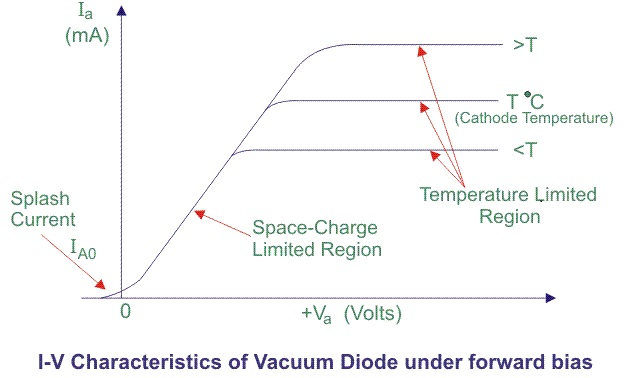
\includegraphics[scale=0.8]{Kennlinie thermische emission}\caption{characteristic curve of thermionic emission}\end{figure}

\section{Conclusion}
Finally it can be said, that the result for the escape work was in the right order of magnitude and therefore quite good. The temperature dependence of the work can  be explained  among others by the mistake of the used model, which didn't account the influence of the space charge density at all, arising when charges leave the metal. This effect is especially notable at low reverse bias voltage and explains the deviation of our measurement data from the linear course in the $U_b\,-\,\text{ln}(I_A)$ diagram at low voltages. We can also understand now the course of emission current, when the reverse bias voltage changes it's sign, which can be explained by by the Schottky-Effect in combination with the space charge density. At even higher voltages the emission current get into saturation. 
Through this experiment we achieved a greater understanding of the physics of thermionic emission and even understood, why in old television devices oxide cathode  diodes were used, because of it's high efficiency.































































\end{document}